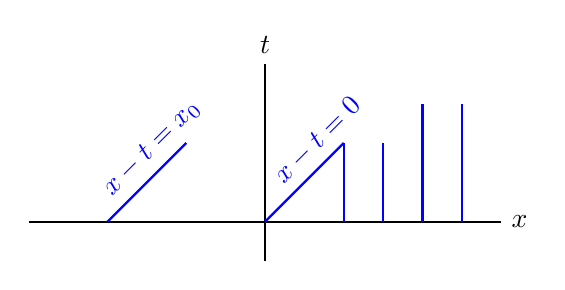
\begin{tikzpicture}
\draw[thick] (-3,0)--(3,0) node[right]{$x$};
\draw[thick] (0,-0.5)--(0,2) node[above]{$t$};


\draw[thick, blue] (-2,0) -- node[above, pos=0.75,sloped]{$x-t=x_0$} (-1,1);

\draw[thick, blue] (0,0) -- node[above, pos=0.85,sloped]{$x-t=0$} (1,1);
\draw[thick, blue] (1,0) --  (1,1);

\draw[thick, blue] (1.5,0) --  (1.5,1);
\draw[thick, blue] (2,0) --  (2,1.5);
\draw[thick, blue] (2.5,0) --  (2.5,1.5);

\end{tikzpicture}